
%% bare_conf.tex
%% V1.4b
%% 2015/08/26
%% by Michael Shell
%% See:
%% http://www.michaelshell.org/
%% for current contact information.
%%
%% This is a skeleton file demonstrating the use of IEEEtran.cls
%% (requires IEEEtran.cls version 1.8b or later) with an IEEE
%% conference paper.
%%
%% Support sites:
%% http://www.michaelshell.org/tex/ieeetran/
%% http://www.ctan.org/pkg/ieeetran
%% and
%% http://www.ieee.org/

%%*************************************************************************
%% Legal Notice:
%% This code is offered as-is without any warranty either expressed or
%% implied; without even the implied warranty of MERCHANTABILITY or
%% FITNESS FOR A PARTICULAR PURPOSE! 
%% User assumes all risk.
%% In no event shall the IEEE or any contributor to this code be liable for
%% any damages or losses, including, but not limited to, incidental,
%% consequential, or any other damages, resulting from the use or misuse
%% of any information contained here.
%%
%% All comments are the opinions of their respective authors and are not
%% necessarily endorsed by the IEEE.
%%
%% This work is distributed under the LaTeX Project Public License (LPPL)
%% ( http://www.latex-project.org/ ) version 1.3, and may be freely used,
%% distributed and modified. A copy of the LPPL, version 1.3, is included
%% in the base LaTeX documentation of all distributions of LaTeX released
%% 2003/12/01 or later.
%% Retain all contribution notices and credits.
%% ** Modified files should be clearly indicated as such, including  **
%% ** renaming them and changing author support contact information. **
%%*************************************************************************


% *** Authors should verify (and, if needed, correct) their LaTeX system  ***
% *** with the testflow diagnostic prior to trusting their LaTeX platform ***
% *** with production work. The IEEE's font choices and paper sizes can   ***
% *** trigger bugs that do not appear when using other class files.       ***                          ***
% The testflow support page is at:
% http://www.michaelshell.org/tex/testflow/



\documentclass[conference]{IEEEtran}
% Some Computer Society conferences also require the compsoc mode option,
% but others use the standard conference format.
%
% If IEEEtran.cls has not been installed into the LaTeX system files,
% manually specify the path to it like:
% \documentclass[conference]{../sty/IEEEtran}





% Some very useful LaTeX packages include:
% (uncomment the ones you want to load)


% *** MISC UTILITY PACKAGES ***
%
%\usepackage{ifpdf}
% Heiko Oberdiek's ifpdf.sty is very useful if you need conditional
% compilation based on whether the output is pdf or dvi.
% usage:
% \ifpdf
%   % pdf code
% \else
%   % dvi code
% \fi
% The latest version of ifpdf.sty can be obtained from:
% http://www.ctan.org/pkg/ifpdf
% Also, note that IEEEtran.cls V1.7 and later provides a builtin
% \ifCLASSINFOpdf conditional that works the same way.
% When switching from latex to pdflatex and vice-versa, the compiler may
% have to be run twice to clear warning/error messages.






% *** CITATION PACKAGES ***
%
\usepackage{cite}
% cite.sty was written by Donald Arseneau
% V1.6 and later of IEEEtran pre-defines the format of the cite.sty package
% \cite{} output to follow that of the IEEE. Loading the cite package will
% result in citation numbers being automatically sorted and properly
% "compressed/ranged". e.g., [1], [9], [2], [7], [5], [6] without using
% cite.sty will become [1], [2], [5]--[7], [9] using cite.sty. cite.sty's
% \cite will automatically add leading space, if needed. Use cite.sty's
% noadjust option (cite.sty V3.8 and later) if you want to turn this off
% such as if a citation ever needs to be enclosed in parenthesis.
% cite.sty is already installed on most LaTeX systems. Be sure and use
% version 5.0 (2009-03-20) and later if using hyperref.sty.
% The latest version can be obtained at:
% http://www.ctan.org/pkg/cite
% The documentation is contained in the cite.sty file itself.






% *** GRAPHICS RELATED PACKAGES ***
%
\ifCLASSINFOpdf
 \usepackage[pdftex]{graphicx}
  % declare the path(s) where your graphic files are
  % \graphicspath{{../pdf/}{../jpeg/}}
  % and their extensions so you won't have to specify these with
  % every instance of \includegraphics
  % \DeclareGraphicsExtensions{.pdf,.jpeg,.png}
\else
  % or other class option (dvipsone, dvipdf, if not using dvips). graphicx
  % will default to the driver specified in the system graphics.cfg if no
  % driver is specified.
  \usepackage[dvips]{graphicx}
  % declare the path(s) where your graphic files are
  % \graphicspath{{../eps/}}
  % and their extensions so you won't have to specify these with
  % every instance of \includegraphics
  % \DeclareGraphicsExtensions{.eps}
\fi
% graphicx was written by David Carlisle and Sebastian Rahtz. It is
% required if you want graphics, photos, etc. graphicx.sty is already
% installed on most LaTeX systems. The latest version and documentation
% can be obtained at: 
% http://www.ctan.org/pkg/graphicx
% Another good source of documentation is "Using Imported Graphics in
% LaTeX2e" by Keith Reckdahl which can be found at:
% http://www.ctan.org/pkg/epslatex
%
% latex, and pdflatex in dvi mode, support graphics in encapsulated
% postscript (.eps) format. pdflatex in pdf mode supports graphics
% in .pdf, .jpeg, .png and .mps (metapost) formats. Users should ensure
% that all non-photo figures use a vector format (.eps, .pdf, .mps) and
% not a bitmapped formats (.jpeg, .png). The IEEE frowns on bitmapped formats
% which can result in "jaggedy"/blurry rendering of lines and letters as
% well as large increases in file sizes.
%
% You can find documentation about the pdfTeX application at:
% http://www.tug.org/applications/pdftex





% *** MATH PACKAGES ***
%
\usepackage{amsmath}
\usepackage{bm} 
% A popular package from the American Mathematical Society that provides
% many useful and powerful commands for dealing with mathematics.
%
% Note that the amsmath package sets \interdisplaylinepenalty to 10000
% thus preventing page breaks from occurring within multiline equations. Use:
%\interdisplaylinepenalty=2500
% after loading amsmath to restore such page breaks as IEEEtran.cls normally
% does. amsmath.sty is already installed on most LaTeX systems. The latest
% version and documentation can be obtained at:
% http://www.ctan.org/pkg/amsmath





% *** SPECIALIZED LIST PACKAGES ***
%
%\usepackage{algorithmic}
% algorithmic.sty was written by Peter Williams and Rogerio Brito.
% This package provides an algorithmic environment fo describing algorithms.
% You can use the algorithmic environment in-text or within a figure
% environment to provide for a floating algorithm. Do NOT use the algorithm
% floating environment provided by algorithm.sty (by the same authors) or
% algorithm2e.sty (by Christophe Fiorio) as the IEEE does not use dedicated
% algorithm float types and packages that provide these will not provide
% correct IEEE style captions. The latest version and documentation of
% algorithmic.sty can be obtained at:
% http://www.ctan.org/pkg/algorithms
% Also of interest may be the (relatively newer and more customizable)
% algorithmicx.sty package by Szasz Janos:
% http://www.ctan.org/pkg/algorithmicx




% *** ALIGNMENT PACKAGES ***
%
%\usepackage{array}
% Frank Mittelbach's and David Carlisle's array.sty patches and improves
% the standard LaTeX2e array and tabular environments to provide better
% appearance and additional user controls. As the default LaTeX2e table
% generation code is lacking to the point of almost being broken with
% respect to the quality of the end results, all users are strongly
% advised to use an enhanced (at the very least that provided by array.sty)
% set of table tools. array.sty is already installed on most systems. The
% latest version and documentation can be obtained at:
% http://www.ctan.org/pkg/array


% IEEEtran contains the IEEEeqnarray family of commands that can be used to
% generate multiline equations as well as matrices, tables, etc., of high
% quality.




% *** SUBFIGURE PACKAGES ***
%\ifCLASSOPTIONcompsoc
%  \usepackage[caption=false,font=normalsize,labelfont=sf,textfont=sf]{subfig}
%\else
%  \usepackage[caption=false,font=footnotesize]{subfig}
%\fi
% subfig.sty, written by Steven Douglas Cochran, is the modern replacement
% for subfigure.sty, the latter of which is no longer maintained and is
% incompatible with some LaTeX packages including fixltx2e. However,
% subfig.sty requires and automatically loads Axel Sommerfeldt's caption.sty
% which will override IEEEtran.cls' handling of captions and this will result
% in non-IEEE style figure/table captions. To prevent this problem, be sure
% and invoke subfig.sty's "caption=false" package option (available since
% subfig.sty version 1.3, 2005/06/28) as this is will preserve IEEEtran.cls
% handling of captions.
% Note that the Computer Society format requires a larger sans serif font
% than the serif footnote size font used in traditional IEEE formatting
% and thus the need to invoke different subfig.sty package options depending
% on whether compsoc mode has been enabled.
%
% The latest version and documentation of subfig.sty can be obtained at:
% http://www.ctan.org/pkg/subfig




% *** FLOAT PACKAGES ***
%
%\usepackage{fixltx2e}
% fixltx2e, the successor to the earlier fix2col.sty, was written by
% Frank Mittelbach and David Carlisle. This package corrects a few problems
% in the LaTeX2e kernel, the most notable of which is that in current
% LaTeX2e releases, the ordering of single and double column floats is not
% guaranteed to be preserved. Thus, an unpatched LaTeX2e can allow a
% single column figure to be placed prior to an earlier double column
% figure.
% Be aware that LaTeX2e kernels dated 2015 and later have fixltx2e.sty's
% corrections already built into the system in which case a warning will
% be issued if an attempt is made to load fixltx2e.sty as it is no longer
% needed.
% The latest version and documentation can be found at:
% http://www.ctan.org/pkg/fixltx2e


%\usepackage{stfloats}
% stfloats.sty was written by Sigitas Tolusis. This package gives LaTeX2e
% the ability to do double column floats at the bottom of the page as well
% as the top. (e.g., "\begin{figure*}[!b]" is not normally possible in
% LaTeX2e). It also provides a command:
%\fnbelowfloat
% to enable the placement of footnotes below bottom floats (the standard
% LaTeX2e kernel puts them above bottom floats). This is an invasive package
% which rewrites many portions of the LaTeX2e float routines. It may not work
% with other packages that modify the LaTeX2e float routines. The latest
% version and documentation can be obtained at:
% http://www.ctan.org/pkg/stfloats
% Do not use the stfloats baselinefloat ability as the IEEE does not allow
% \baselineskip to stretch. Authors submitting work to the IEEE should note
% that the IEEE rarely uses double column equations and that authors should try
% to avoid such use. Do not be tempted to use the cuted.sty or midfloat.sty
% packages (also by Sigitas Tolusis) as the IEEE does not format its papers in
% such ways.
% Do not attempt to use stfloats with fixltx2e as they are incompatible.
% Instead, use Morten Hogholm'a dblfloatfix which combines the features
% of both fixltx2e and stfloats:
%
% \usepackage{dblfloatfix}
% The latest version can be found at:
% http://www.ctan.org/pkg/dblfloatfix




% *** PDF, URL AND HYPERLINK PACKAGES ***
%
%\usepackage{url}
% url.sty was written by Donald Arseneau. It provides better support for
% handling and breaking URLs. url.sty is already installed on most LaTeX
% systems. The latest version and documentation can be obtained at:
% http://www.ctan.org/pkg/url
% Basically, \url{my_url_here}.




% *** Do not adjust lengths that control margins, column widths, etc. ***
% *** Do not use packages that alter fonts (such as pslatex).         ***
% There should be no need to do such things with IEEEtran.cls V1.6 and later.
% (Unless specifically asked to do so by the journal or conference you plan
% to submit to, of course. )


% correct bad hyphenation here
\hyphenation{op-tical net-works semi-conduc-tor GYOU-KOU}

\newcommand\rsquo{'}
          % Astronomical Journal 
\newcommand\aj{{AJ}}% 
          % Astronomical Journal 
\newcommand\araa{{ARA\&A}}% 
          % Annual Review of Astron and Astrophys 
\newcommand\apj{{ApJ}}% 
          % Astrophysical Journal 
\newcommand\apjl{{ApJ}}% 
          % Astrophysical Journal, Letters 
\newcommand\apjs{{ApJS}}% 
          % Astrophysical Journal, Supplement 
\newcommand\ao{{Appl.~Opt.}}% 
          % Applied Optics 
\newcommand\apss{{Ap\&SS}}% 
          % Astrophysics and Space Science 
\newcommand\aap{{A\&A}}% 
          % Astronomy and Astrophysics 
\newcommand\aapr{{A\&A~Rev.}}% 
          % Astronomy and Astrophysics Reviews 
\newcommand\aaps{{A\&AS}}% 
          % Astronomy and Astrophysics, Supplement 
\newcommand\azh{{AZh}}% 
          % Astronomicheskii Zhurnal 
\newcommand\baas{{BAAS}}% 
          % Bulletin of the AAS 
\newcommand\jrasc{{JRASC}}% 
          % Journal of the RAS of Canada 
\newcommand\memras{{MmRAS}}% 
          % Memoirs of the RAS 
\newcommand\mnras{{MNRAS}}% 
          % Monthly Notices of the RAS 
\newcommand\pra{{Phys.~Rev.~A}}% 
          % Physical Review A: General Physics 
\newcommand\prb{{Phys.~Rev.~B}}% 
          % Physical Review B: Solid State 
\newcommand\prc{{Phys.~Rev.~C}}% 
          % Physical Review C 
\newcommand\prd{{Phys.~Rev.~D}}% 
          % Physical Review D 
\newcommand\pre{{Phys.~Rev.~E}}% 
          % Physical Review E 
\newcommand\prl{{Phys.~Rev.~Lett.}}% 
          % Physical Review Letters 
\newcommand\pasp{{PASP}}% 
          % Publications of the ASP 
\newcommand\pasj{{PASJ}}% 
          % Publications of the ASJ 
\newcommand\qjras{{QJRAS}}% 
          % Quarterly Journal of the RAS 
\newcommand\skytel{{S\&T}}% 
          % Sky and Telescope 
\newcommand\solphys{{Sol.~Phys.}}% 
          % Solar Physics 
\newcommand\sovast{{Soviet~Ast.}}% 
          % Soviet Astronomy 
\newcommand\ssr{{Space~Sci.~Rev.}}% 
          % Space Science Reviews 
\newcommand\zap{{ZAp}}% 
          % Zeitschrift fuer Astrophysik 
\newcommand\nat{{Nature}}% 
          % Nature 
\newcommand\iaucirc{{IAU~Circ.}}% 
          % IAU Cirulars 
\newcommand\aplett{{Astrophys.~Lett.}}% 
          % Astrophysics Letters 
\newcommand\apspr{{Astrophys.~Space~Phys.~Res.}}% 
          % Astrophysics Space Physics Research 
\newcommand\bain{{Bull.~Astron.~Inst.~Netherlands}}% 
          % Bulletin Astronomical Institute of the Netherlands 
\newcommand\fcp{{Fund.~Cosmic~Phys.}}% 
          % Fundamental Cosmic Physics 
\newcommand\gca{{Geochim.~Cosmochim.~Acta}}% 
          % Geochimica Cosmochimica Acta 
\newcommand\grl{{Geophys.~Res.~Lett.}}% 
          % Geophysics Research Letters 
\newcommand\jcp{{J.~Chem.~Phys.}}% 
          % Journal of Chemical Physics 
\newcommand\jgr{{J.~Geophys.~Res.}}% 
          % Journal of Geophysics Research 
\newcommand\jqsrt{{J.~Quant.~Spec.~Radiat.~Transf.}}% 
          % Journal of Quantitiative Spectroscopy and Radiative Trasfer 
\newcommand\memsai{{Mem.~Soc.~Astron.~Italiana}}% 
          % Mem. Societa Astronomica Italiana 
\newcommand\nphysa{{Nucl.~Phys.~A}}% 
          % Nuclear Physics A 
\newcommand\physrep{{Phys.~Rep.}}% 
          % Physics Reports 
\newcommand\physscr{{Phys.~Scr}}% 
          % Physica Scripta 
\newcommand\planss{{Planet.~Space~Sci.}}% 
          % Planetary Space Science 
\newcommand\procspie{{Proc.~SPIE}}% 
          % Proceedings of the SPIE 
\let\astap=\aap 
\let\apjlett=\apjl 
\let\apjsupp=\apjs 
\let\applopt=\ao 
    
\begin{document}
%
% paper title
% Titles are generally capitalized except for words such as a, an, and, as,
% at, but, by, for, in, nor, of, on, or, the, to and up, which are usually
% not capitalized unless they are the first or last word of the title.
% Linebreaks \\ can be used within to get better formatting as desired.
% Do not put math or special symbols in the title.
\title{48-petaflops  global simulation of planetary rings on
Sunway TaihuLight  and GYOUKOU}


% author names and affiliations
% use a multiple column layout for up to three different
% affiliations
%% \author{\IEEEauthorblockN{Michael Shell}
%% \IEEEauthorblockA{School of Electrical and\\Computer Engineering\\
%% Georgia Institute of Technology\\
%% Atlanta, Georgia 30332--0250\\
%% Email: http://www.michaelshell.org/contact.html}



%% \author{\IEEEauthorblockN{Michael Shell}
%% \IEEEauthorblockA{School of Electrical and\\Computer Engineering\\
%% Georgia Institute of Technology\\
%% Atlanta, Georgia 30332--0250\\
%% Email: http://www.michaelshell.org/contact.html}
%% \and
%% \IEEEauthorblockN{Homer Simpson}
%% \IEEEauthorblockA{Twentieth Century Fox\\
%% Springfield, USA\\
%% Email: homer@thesimpsons.com}
%% \and
%% \IEEEauthorblockN{James Kirk\\ and Montgomery Scott}
%% \IEEEauthorblockA{Starfleet Academy\\
%% San Francisco, California 96678--2391\\
%% Telephone: (800) 555--1212\\
%% Fax: (888) 555--1212}}

% conference papers do not typically use \thanks and this command
% is locked out in conference mode. If really needed, such as for
% the acknowledgment of grants, issue a \IEEEoverridecommandlockouts
% after \documentclass

% for over three affiliations, or if they all won't fit within the width
% of the page, use this alternative format:
% 
\author{\IEEEauthorblockN{
    Masaki Iwasawa\IEEEauthorrefmark{1},
    Daisuke Namekata\IEEEauthorrefmark{1},
    Ryo Sakamoto\IEEEauthorrefmark{2},
    Takashi Nakamura\IEEEauthorrefmark{2},
    Yasuyuki Kimura\IEEEauthorrefmark{3},
    Keigo Nitadori\IEEEauthorrefmark{1},\\
    Long Wang\IEEEauthorrefmark{1},
    Miyuki Tsubouchi\IEEEauthorrefmark{1},
    Jun Makino\IEEEauthorrefmark{4},
    Zhao Liu\IEEEauthorrefmark{5},
    Haohuan Fu\IEEEauthorrefmark{6},
    Guangwen Yang\IEEEauthorrefmark{7}}
\IEEEauthorblockA{\IEEEauthorrefmark{1}RIKEN CCS\\
7--1--26 Minatojima-minami-machi, Chuo-ku, Kobe, Hyogo,  650--0047, Japan\\
Email: masaki.iwasawa@riken.jp}
\IEEEauthorblockA{\IEEEauthorrefmark{2}
PEZY Computing K. K.\\
1--11 Ogawa-machi, Chiyoda-ku, Tokyo,  101--0052, Japan\\
Email: sakamoto@pezy.co.jp}
\IEEEauthorblockA{\IEEEauthorrefmark{3}
ExaScaler Inc.\\
2--1 Ogawa-machi, Chiyoda-ku, 101--0052 Tokyo, Japan\\
Email: yasuyuki@exascaler.co.jp}
\IEEEauthorblockA{\IEEEauthorrefmark{4}
  Kobe University\\
  1--1, Rokkodai-cho, Nada-ku, Kobe, 657--8501, Japan\\
  Email: jmakino@people.kobe-u.ac.jp}
\IEEEauthorblockA{\IEEEauthorrefmark{5}
National Supercomputing Center in Wuxi\\
Wuxi, China\\
Email:liuzhao@mail.nsccwx.cn}
\IEEEauthorblockA{\IEEEauthorrefmark{6}
Department of Earth System Science, Tsinghua University\\
Beijing, China\\
Email:haohuan@tsinghua.edu.cn}
\IEEEauthorblockA{\IEEEauthorrefmark{7}
Department of Computer Science and Technology, Tsinghua University\\
Beijing, China\\
Email:ygw@tsinghua.edu.cn}}




% use for special paper notices
%\IEEEspecialpapernotice{(Invited Paper)}




% make the title area
\maketitle

% As a general rule, do not put math, special symbols or citations
% in the abstract
\begin{abstract}
  In this paper, we report an implementation and measured performances
  of an extreme-scale global simulation code for planetary rings on
  Sunway TaihuLight and PEZY-SC2 GYOUKOU systems.
  The numerical algorithm is the parallel Barnes-Hut tree algorithm,
  which has been used in many large-scale astrophysical particle-based
  simulations including several awardees of the Gordon Bell
  Prize. However, extremely large numbers of cores of the systems
  used (10M on TaihuLight and 16M on GYOUKOU)  and their relatively poor
  memory and network bandwidth pose new challenges. We describe 
  new algorithms introduced to achieve high efficiency on machines
  with low memory bandwidth.  The measured
  performance is 47.9 and 10.6 Pflops, on TaihuLight and GYOUKOU
  (efficiency  40\% and 23.5\%). 
\end{abstract}

% no keywords




% For peer review papers, you can put extra information on the cover
% page as needed:
% \ifCLASSOPTIONpeerreview
% \begin{center} \bfseries EDICS Category: 3-BBND \end{center}
% \fi
%
% For peerreview papers, this IEEEtran command inserts a page break and
% creates the second title. It will be ignored for other modes.
\IEEEpeerreviewmaketitle

\section{Justification for ACM Gordon Bell Prize}

% 50 wiords max

We have achieved 40\% and 23.5\% of the theoretical peak performance,
or 47.9 Pflops and 10.6 Pflops, on the Sunway TaihuLight system and
the GYOUKOU system with PEZY-SC2 processors, for the simulation of
planetary rings.  We have incorporated many new techniques to achieve
high efficiency on these systems.



\section{Performance Attributes}

  \begin{tabular}{ll}
    \hline
    Category of achievement&  scalability,\\
                            &time-to-solution,\\
                           &peak performance\\
    Type of method used & Explicit with\\
                        &long-range interaction\\    
    Results reported on the basis of&  whole application\\
     Precision reported &  mixed precision\\
     System scale & results measured on \\
                  &full-scale system\\
    Measurement mechanism &   FLOP count\\

 \hline
\end{tabular}

  \section{Overview of the Problem}
  \label{sect:overview}

%    description of the problem and its importance, in terms
  %    understandable to a non-specialist (1 p max)

  

Saturn's ring was first observed by Galileo Galilei in 1610. For more
than three centuries, it had been the only known ring system within
our solar system. In 1977, rings of Uranus were found through
occultation observations from an aircraft, and then in 1979 rings of
Jupiter by Voyager 1 and in 1989 those of Neptune by Voyager 2.  Very
recently, it turned out that some of minor planets also have
rings. The first distinctive example is 10199 Chariklo, whose orbit is
between those of Saturn and Uranus (and thus one of Centaurs). There
are probably more Centaurs with rings.

Thus, quite recently, a wide variety of ring systems have been found.
How these rings were formed and have evolved is an important question
in planetary science, and large-scale, global simulation, if possible,
would help greatly to advance our understanding.

Planetary rings are usually at the radii around the Roche limit. Thus,
mutual gravity between particles does not easily lead to the formation
of new satellites, but is important enough to form spiral waves
(``wakes'') in very small scales, which increase the effective
viscosity and should enhance the radial transport of the angular
momentum. On the other hand, the actual ring system seems to consist
of very large number of narrow rings, separated with distinct gaps. It
is believed that these gaps are maintained by high-order resonances
with small embedded satellites (so-called moonlets), but whether or
not such gaps can be formed and maintained by resonances has not been
fully understood.

Up to now, most of simulations of ring structures have been local
ones, in which a small patch  was cut out from the ring and simulated
under an assumption of local Hill approximation and a periodic
boundary condition\cite{WisdomTremaine1988}. Rein and Latter\cite{ReinLatter2013}
performed ``Large-scale'' simulation of viscous
overstability in Saturn's rings, using up to 204,178 particles and up
to 10,000 orbits using this local approach.  Because very long
simulations are necessary, the number of particles has been
small. They used {\tt REBOUND}\cite{ReinLiu2012}, an MPI-parallel
$N$-body simulation code.


Michikoshi and Kokubo\cite{MichikoshiKokubo2017} performed global simulations of rings with
the largest number of particles reported so far. They used 300M particles to
model two narrow rings of Chariklo. They have developed their parallel
code using the framework we developed, FDPS\cite{Iwasawaetal2016}. 

\section{Current State of the Art}


%   quantitative discussion of current SoA, with emphasis on
%   performance-related aspects  (1 p max)   

% GreeM 1.800e10 particle steps/sec

As we stated in the previous section, almost all previous studies of
planetary rings adopted so-called ``local'' approximation, in which
only a small patch of a ring is simulated assuming periodic boundary
condition in both radial and azimuthal directions,
with a cut-off length in the self gravitating force. 

Michikoshi and Kokubo\cite{MichikoshiKokubo2017} performed global
simulations of rings with 300M particles, using
FDPS\cite{Iwasawaetal2016}. They so far followed the system only for
10 orbital periods.

The total calculation cost is roughly proportional to number of
particles multiplied by the number of orbital periods followed, since
the calculation cost per timestep is $O(N \log N)$ when Barnes and Hut
tree algorithm is used and the number of timestep required for ring
simulations is essentially independent of the number of
particles. Thus, we can conclude that the size of state-of-the-art
simulations of planetary rings is around $10^9$ particle-orbits, or
around $10^{12}$ particle-steps.

We should note that even though the simulations so far done in this
field is relatively small, that does not mean there is no need or
possibilities for larger scale simulations. If we want to model the
global structures of rings, we cannot rely on local treatment. For
example, the effect of resonances with small satellites can only be
studied using global simulations. On the other hand, the number of
particles one need for global simulations, even  for a very narrow
radial range, is very large. For example, consider the A ring of Saturn
with the radius of around $1.3\times 10^5$ km. The typical radius
of ring particles is 6~m\cite{ZEBKER1985531}, and the optical depth of
the ring is around unity. Thus, we need $10^4$ particles per km$^2$ 
or around $10^{12}$ particles for the radial range of 100
km. With this radial range, we can model many of fine features observed
by Cassini directly.

If we could use particles with larger radial size, we could reduce the number
of particles required significantly. However, that would change the
viscous diffusion timescale of the ring, and thus what would be
observed. It is necessary to perform
simulations with particles of real physical radius, which would require
at least $10^{16}$ and ideally $10^{19}$ particle steps.

In other fields of astrophysics, very large simulations have been
performed. For example, Ishiyama\cite{Ishiyama2014} used $4096^3$
particles to follow the formation and growth of dark matter halos of
smallest scales. This simulation corresponds to  $10^{16}$ particle
steps. Part of this calculation was performed on K computer. The
performance of K computer is $4.0\times 10^{10}$ particle steps per
second on the entire K computer, or 60,000 particle step per second
per core for a processor core with the theoretical peak performance of
16 Gflops\cite{Ishiyamaetal2012}. The efficiency they achieved is 55\%
of the theoretical peak. 


The algorithms used in large-scale $N$-body simulations are rather
similar, and that means they are well studied and close to optimal.
 All of them use domain
decomposition and Barnes and Hut tree algorithm. For domain
decomposition, several variations have been used, such as
Orthogonal Recursive Bisection\cite{Salmon1990}, Hashed Oct
Tree\cite{WarrenSalmon1992}, Multisection\cite{Makino2004}.


Efficient implementations on large-scale GPGPU clusters
exist\cite{Hamadaetal2009, PortegiesZwartetal2014, Bedorfetal2014}.
B{\'e}dorf {\it et al}.~performed the simulation of Milky Way Galaxy
using $2.42 \times 10^{11}$ particles. The achieved performance is
24.77 Pflops on ORNL Titan, and one timestep took 5.5 seconds. Thus
they have achieved the performance of $4.4 \times 10^{10}$ particle
steps per seconds. The theoretical peak performance of Titan is 73.2
Pflops in single precision. Thus, the achieved efficiency is 33.8\%.

So far, there is no report on the implementation and performance of
parallel tree algorithm on processors with a heterogeneous
architecture such as Sunway TaihuLight or GYOUKOU.  In this paper, we
present the result of our effort to implement the parallel tree
algorithm on them.


\section{Sunway TaihuLight and GYOUKOU}

In this section, we briefly describe the features of the Sunway
TaihuLight system and GYOUKOU. The former consists of 40960 Sunway 26010
processors, and the latter 13312 PEZY-SC2 processors. 

One SW26010 processor consists of four core groups (CGs), each with one
management processing element (MPE) and 64 computing processing elements (CPEs). 
Both MPE and CPE are 64-bit RISC cores. MPE has L1 cache
memories for  both instructions and data, and also L2 data cache. On
the other hand, each CPE has L1 instruction cache and 64KB of local
data memory. CPEs can communicate with the main memory through DMA.
Each CPE can initiate multiple asynchronous DMA operations. 

Each core group is connected to 8 GiB DDR3 DRAM memory with the theoretical
peak transfer rate of 34 GB/s. The processor runs at the clock
frequency of 1.45 GHz, and each core (both MPE and CPE) can perform
four double precision FMA operations. Thus, the theoretical peak
performance of one processor is 3016 Gflops and that of one CG is 754
Gflops. Thus, even when we use the nominal number for DRAM bandwidth,
the B/F ratio is only 0.045. This is less than 1/10 of the number for
K computer.

Compared to that of K computer, the network is also  weak,
with the total bandwidth of around 10 GB/s per node. This is about the
same as the performance of a single link of 6D mesh/torus network of K
computer. Since the SW processor is around 25 times faster than the
SPARC64 processor of K~computer, the relative network bandwidth is
different by  more than two orders of magnitudes.

One PEZY-SC2 processor chip consists of  2048 processors (64
of them are disabled and the available number of processors is
1984). Each processor can perform 1, 2 and 4 multiply-and-add
operation for FP64, FP32, and FP16 data. For FP32 and FP16, 2- and
4-way SIMD operations are performed.  With the clock speed of 700MHz,
the theoretical peak speed is 2.8, 5.6 and 11.1 Tflops, for FP64, FP32 and
FP16, respectively. At present, each SC2 processor chip have 4 channels of
DDR4 memory, for the peak throughput of 76.8 GB/s. Thus B/F is 0.027.

They have three levels of shared cache, but without
coherency. Instead, they have explicit cache flush instructions to each
levels. Two processors share L1D, and 16 processors L2D, and all
processors LLC. Each processor runs either four or eight threads
simultaneously. Thus, it is relatively easy to hide the  latency of
the arithmetic units and L1D.

In the original design, each SC2 processor chip had six MIP64 cores,
which were supposed to run the operating system and main body of the
application programs. Unfortunately, they are currently disabled, and
operating system and application programs run on the frontend  Xeon~D-1571
processor. Each Xeon~D hosts eight SC2 processors. Thus, the
performance ratio between Xeon~D and SC2 is close to 100.
Moreover, these eight SC2 are connected to Xeon~D through single PCIe
Gen3 16-lane channel. Thus, the peak data transfer speed between one
SC2 and Xeon~D is 2 GB/s, for the peak speed of 2.8 Tflops.


%
% Xeon-D 1571 1.3GHz 16 Broadwell core = 333 GF peak, 42GF/2cores
In summary, TaihuLight and GYOUKOU share the following
characteristics:

\begin{enumerate}



\item Very large performance ratio between ``general-purpose''
  and ``computing'' cores, close to 1:100.
\item  Very small memory  B/F numbers, around 0.03.
\item  Even smaller network B/F numbers, 0.006 or 0.001.
\item Very large number of MPI processes, 160k  or 10k.
\item Very large number of ``computing'' cores per MPI process, 64 or 1984.  
\end{enumerate}

Just one of these characteristics makes it very difficult to achieve
reasonable performance for particle-based simulations using previously
known parallelization algorithms. In the next section, we describe the
new algorithms we implemented to achieve good performance on these systems.



\section{Innovations Realized}
\label{sect:innovation}
%   what the innovations are and how they were achieved (2 pp max)

  \subsection{Overview of Innovations}

  
In this section, we describe the new innovations we made in order to
utilize TaihuLight and GYOUKOU for the simulations of self-gravitating
planetary rings. The following is the list of innovations.


\begin{enumerate}
\item The reuse of the interaction list over multiple timesteps.
\item Elimination of  the global all-to-all communication.
\item ``Semi-dynamic'' load balance between computing cores.
\item Optimizations specific to the ring geometry.
\end{enumerate}  

In the rest of this section, we briefly describe these new innovations.

\subsection{The reuse of the interaction list}
\label{subsec:list}


The following gives the usual steps for highly parallel code for
self-gravitating particle system:

\begin{enumerate}

  \item Perform domain decomposition.
  \item Exchange particles so that particles belong to appropriate domains.
  \item Perform interaction calculation using fast algorithm such as
    Barnes-Hut tree.
  \item Integrate the orbits of particles.
  \item Go back to step 1.

\end{enumerate}

In the case of approaches with local essential tree, step (3) consists
of the following substeps:

\begin{description}

\item{(3a)} Construct the ``local'' tree structure from particles in
  the domain.
\item{(3b)} Collect the information necessary for the calculation of
  interaction from other processes (so called local essential tree).
\item{(3c)} Construct the ``global'' tree from the collected information.
\item{(3d)} For small groups of particles, traverse the tree and
  calculate the interaction. Repeat this for all groups.
\end{description}
In the original algorithm\cite{BarnesHut1986}, the traversal of the
tree is done for each particle, and force calculation is done during
the traversal. However, on almost all modern implementation, following
the idea of Barnes\cite{Barnes1990}, tree traversal are done for
groups of neighboring particles, which are constructed using the tree
structure itself. During the traversal for a group, the list of
particles and tree nodes which exert the force on this group of
particles is constructed, and actual force calculation is done through
the double loop over particles in the group and those in the
list. This structure makes it possible to use vector pipelines, scalar
SIMD units, and even special-purpose computers\cite{Makino1991c} with
high efficiency. For GPGPUs, the extension of this algorithm, in which
multiple lists are constructed and then sent to GPGPU, is
used\cite{Hamadaetal2009}.

This approach does not work well on TaihuLight or GYOUKOU, because of
the low performance of general-purpose core and limited memory bandwidth. 
The
performance we can achieve with either approach for ring simulation on
these machines is less than 1\%.
Thus, it is necessary to reduce the cost of tree construction and tree
traversal, and we achieved this by using the same interaction lists
over multiple timesteps. We call this method the persistent
interaction list method.

The idea behind this method is essentially the same as that for
the  neighbor-list method used in many simulation codes for particles
with short-range  interactions. 

By using this persistent interaction list, we can reduce the
calculation cost of the part other than the interaction calculation
drastically. While we are using the same interaction lists, we skip the
domain decomposition, exchange of particles, construction of the local
tree. We still need to update the physical quantities of the nodes of
the tree, since particles move at each timestep.
We first update the information of the nodes of
the local tree. Then,
using the list of nodes for the local essential tree, the
communication between the nodes is performed. Finally, the physical
quantities of the global tree are updated, and the force calculation is
performed using this updated global tree and the persistent
interaction list.

The most time-consuming part of the tree construction is the
sorting. In the case of TaihuLight, we implemented the parallel sample sort
algorithm\cite{cmsort} on CPEs. In the case of GYOUKOU, the sorting is currently
performed on Xeon~D host processor.

We have ported all operations in timesteps in which the interaction
list is used (list-reusing steps), except for MPI functions for
communication, to CPEs (TaihuLight) or SC2 processors (GYOUKOU). For
the timestep in which the interaction list is constructed
(list-constructing step), most of operations are still done on Xeon~D
in the case of GYOUKOU.

\subsection{Tree and Domain structures on Cylindrical Coordinate}
\label{subsec:cylcoord}

We want to model a relatively narrow ring, and this means the usual
domain decomposition in Cartesian coordinates can cause serious
problems. Figure~\ref{fig:domain_cart} illustrate the problem. We
can see the domains near the $y$ axis are very elongated. This
irregular shape of domains results in the increase of communication
between processes, and thus serious degradation in the efficiency. 

\begin{figure}
  \centering 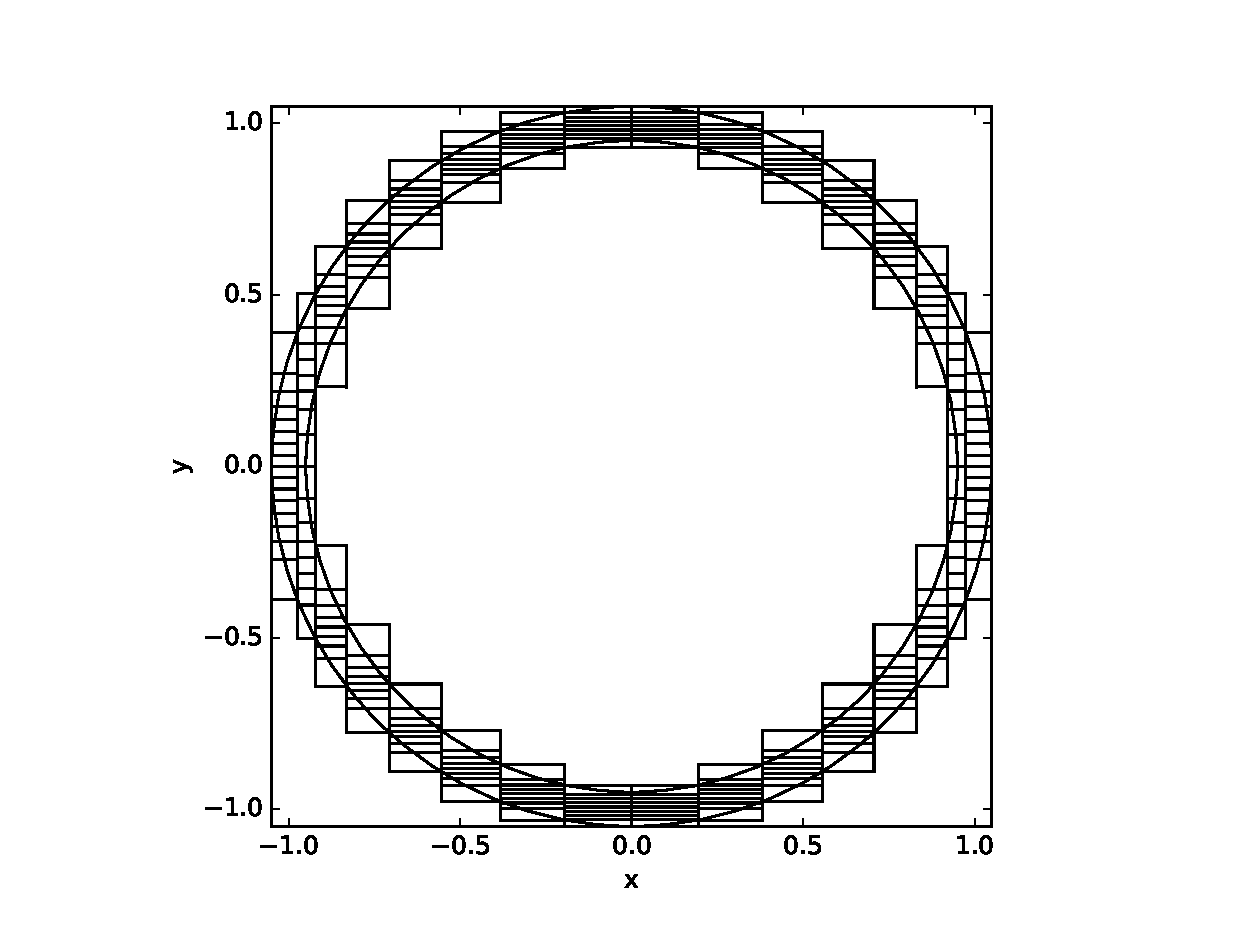
\includegraphics[width=8cm,clip]{./fig/domain_cart.eps}
  \caption{Schematic figure of domain decomposition by the multisection
    method in $x$-$y$ coordinate. Domains are divided by $16 \times 8$.}
  \label{fig:domain_cart}
\end{figure}

\begin{figure}
  \centering
    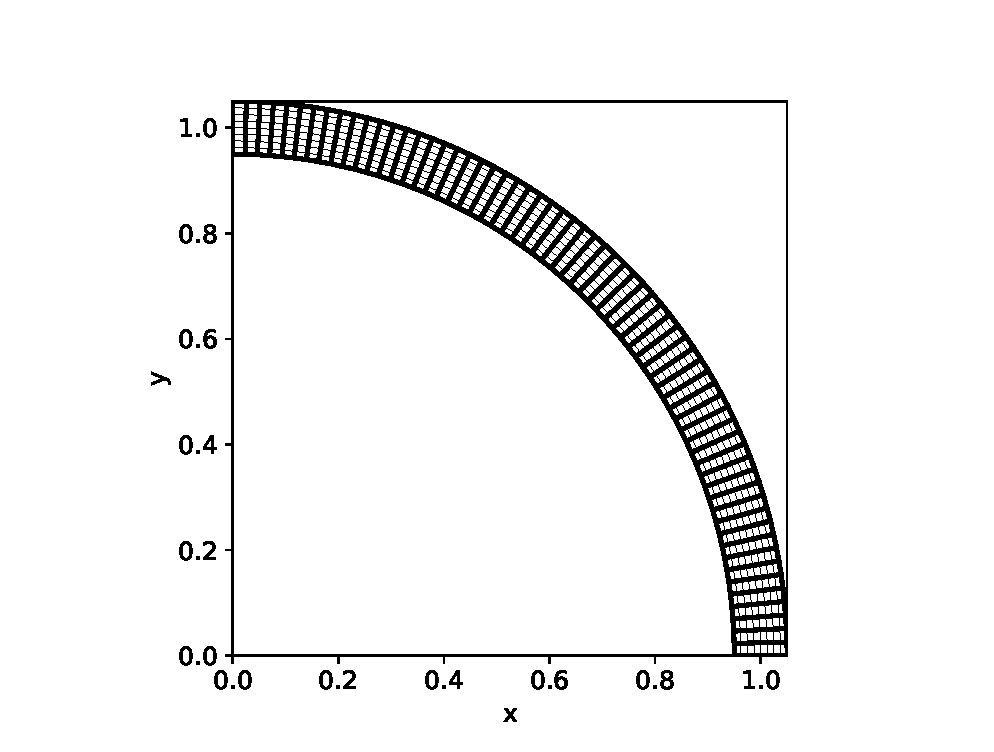
\includegraphics[width=8cm,clip]{./fig/domain_cyl.eps}
  \caption{Schematic figure of domain decomposition by the multisection
    method in cylindrical coordinate. Domains are divided by $4 \times 32$.}
  \label{fig:domain_cyl}
\end{figure}

We can avoid this problem, if we apply the domain decomposition 
in the  cylindrical coordinates (figure  \ref{fig:domain_cyl}).
Note that we can also use the  cylindrical coordinates for the
construction of the tree.  Since
the ring is narrow, the local distance $s$ in the Cartesian coordinates
$(x, y, z)$ can be approximated by that in cylindrical coordinates
($r$, $\phi$, $z$).
\begin{equation}
  \label{eq:metric}
  ds^2 = dx^2 + dy^2 + dz^2 \sim d\phi ^2 + dr^2 + dz^2,
\end{equation}
when $r \sim 1$. Thus,
we can use the cylindrical coordinate
for domain decomposition and tree
construction and even for the tree traversal,  without any modification of the algorithm or program
itself. The actual interaction calculation is faster in Cartesian
coordinates and thus Cartesian coordinates is used.


\subsection{Coordinate rotation}
\label{subsec:exptcl}

The simulation of ring with very large number of processes poses
new challenges. As we increase the number of processes, the size of
the domains becomes smaller. On the other hand, the timestep does not
become much smaller even when we increase the total number of
particles, since the random velocities of ring particles become
smaller when we increase the number of particles. Thus, the distance
that particles move can be comparable or even larger than the domain
size, resulting in the increase in the amount of  communication.

We can ``solve'' this problem by the rotation of  the coordinates and domain
structure, so that particles do not move much. If we rotate the
coordinates at the speed of Kepler rotation at the center of the ring,
particles at the center of the ring do not move much. Particles at
other radial positions still move, but the speed becomes much smaller
than that of the Kepler rotation. Thus, communication due to Kepler
rotation can be almost eliminated.


\subsection{Elimination of all-to-all communication}
\label{subsec:exlet}

%% \begin{figure}
%%   \centering 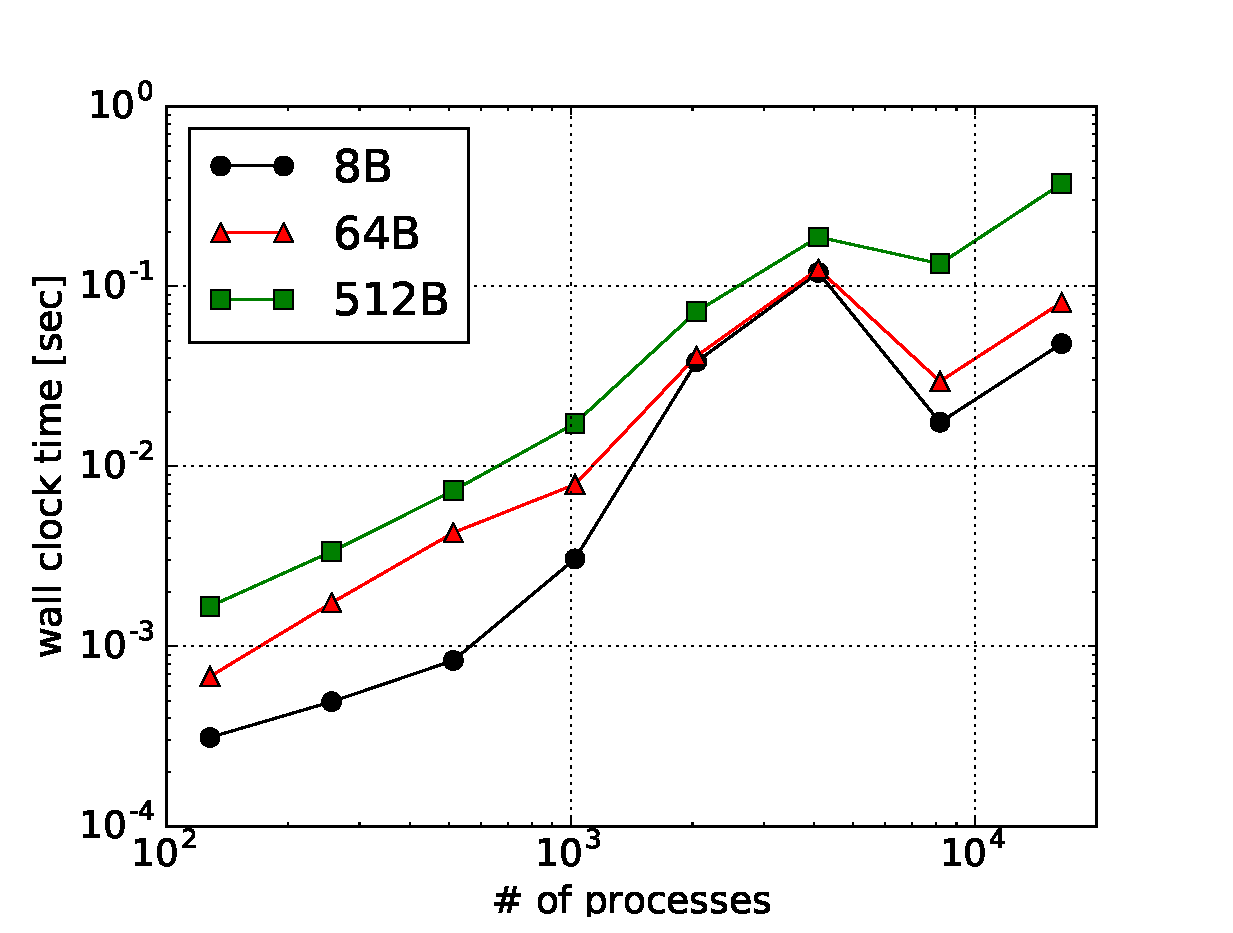
\includegraphics[width=8cm,clip]{./fig/comm_np-wtime.eps}
%%   \caption{Wall clock time for {\tt MPI\_Alltoall} against the number of processors.}
%%   \label{fig:comm_np-wtime}
%% \end{figure}

%% \begin{figure}
%%   \centering
%%   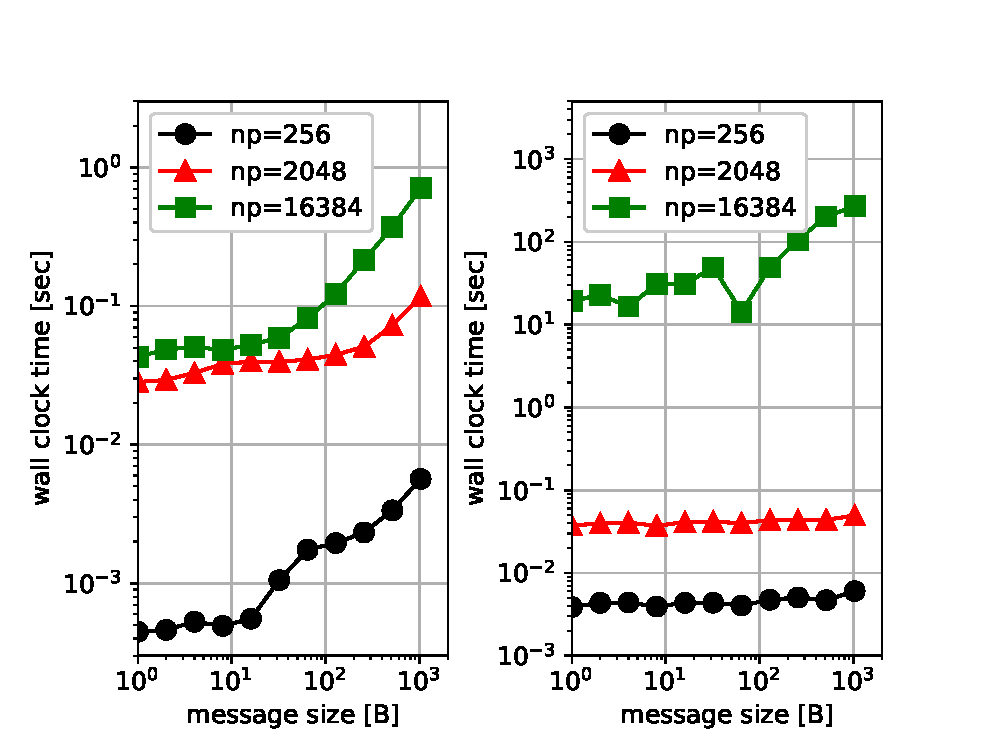
\includegraphics[width=8cm,clip]{./fig/comm_msize-wtime.eps}
%%   \caption{Wall clock time for {\tt MPI\_Alltoall} against the size of the message sent per process.}
%%   \label{fig:comm_msize-wtime}
%% \end{figure}

In FDPS, the exchange of LET (local essential tree) data is done
though a single call to the {\tt MPI\_Alltoallv} function.  This
implementation works fine even for full-node runs on K computer, but
becomes problematic on systems with relatively weak network like
TaihuLight and GYOUKOU. We can eliminate this all-to-all communication, by
constructing the ``tree of domains'' locally and let only higher-level
information be sent to distant processes.

In the current implementation specialized to narrow rings, we
implemented a very simple two-level tree, in which the second-level
tree nodes have all processes in the radial direction. For example, if we
have a process grid of (1000, 10), where 1000 in angular and 10 in
radial direction, 10 domains in the radial direction are combined to
one tree node, resulting in 1000 second-level nodes. Only these 1000
nodes exchange their center-of-mass information. All LET information
other than these center-of-mass data of second-level nodes are sent
either to other second-level nodes (and then broadcast to
lower-level nodes) or sent directly to lower-level nodes.

In this implementation, there is still one global communication in the
angular direction, but we can use {\tt MPI\_Allgather} since only the
top-level data are sent. Thus the reduction in the communication was
quite significant.


\subsection{Load Balance among computing cores}
\label{subsec:force}

In our current implementation, interaction lists are created at the
list-construction step, and are reused for several steps. The total
number of lists in one MPI process is around $10^5$, and we need to
use 64 or 1984 computing cores efficiently for them.
If we just assign a fixed number of lists to cores, random variation
of the list length can result in large load imbalance. Therefore, some
load balance strategy is necessary. We applied the following simple algorithm.

\begin{enumerate}
  
\item Sort the interaction lists by their length.

\item Assign the longest 64 lists on 64 CPEs (in case of TaihuLight).

\item For each remaining list, assign it to the the CPE with the
  shortest total calculation cost.
  
\end{enumerate}

Since the calculation time of cores is quite predictable, this
algorithm works very well.

In the case of GYOUKOU, we further improve the load balance by using
multiple cores which share the cache for 
one interaction list.

\subsection{Interaction Kernel}

In the case of TaihuLight, we found the compiler-generated code for
the interaction kernel, even when SIMD operations are used, does not
give very good performance. We rewrite the interaction kernel fully in
the assembly language, with hand-unroll and careful manual scheduling. As
a result, we achieved more than 50\% of the theoretical peak
performance for the kernel.

We have applied similar optimization also
on GYOUKOU. In addition, on GYOUKOU we used single-precision
calculation for the interaction kernel. In order to avoid the large
roundoff at the first subtraction of the position vectors, after the
interaction list is constructed, both positions and velocities are
shifted with the new origin at the position of one of the particles which share the
interaction list. After this shifting, positions and velocities are
converted to single precision, and actual interaction calculation is
done using single-precision SIMD operations.


\section{How Performance Was Measured}

% (Note that preference is given to performance actually measured [not
% projected], based on the entire application [including I/O] and with
% uniform precision.  Explain in detail if any portion of total
% runtime was not included in the measurements, if and where different
% precisions were used, or any attributes listed in Section 3 as
% “other”).  what application(s) was used to measure performance (1
% p max) system and environment where performance was measured (1 p
  % max)

To measure the performance, we measure the time for 64 timesteps,
including the time for  diagnostics. 
The
execution time is measured by the MPI wallclock timer, and operation
count is from the counted number of interactions
calculated. Equation~\ref{eq:interation}  gives the definition of the
particle-particle interaction. 
{%\scriptsize
\begin{equation}
  \bm F_{ij} = \begin{cases} G \dfrac{m_i m_j}
    {r_{ij}^3} \bm r_{ij} & \left(r_{ij} > r_\text{coll} \right)
    \\
    \Biggl[  G \dfrac{m_i m_j} {r_\text{coll}^3}  + \dfrac{m_j}{m_i
        + m_j}  \times \\ \qquad  \left(      \kappa \dfrac{r_{ij} -
        r_\text{coll}}{r_{ij}}    + \eta \dfrac{\bm r_{ij} \cdot \bm
        v_{ij}}{r_{ij}^2}    \right) \Biggr] \bm r_{ij} & \left(
    r_{ij} \le r_\text{coll} \right) \end{cases}
  \label{eq:interation} 
\end{equation}
}
with
$\bm r_{ij} = \bm r_j - \bm r_i$, $\bm v_{ij} = \bm v_j - \bm v_i$,
$r_{ij} = \| \bm r_{ij} \|$

%% \begin{equation} 
%%   \label{eq:interation}
%%   {\mathbf F_{ij}}= \begin{cases}
%%     -G\frac{m_im_j}{r_{ij}^3}{\mathbf r_{ij}},& (r_{ij}>r_{coll})\\
%%     -\eta{\mathbf v_{r,ij}} - \kappa(r_{ij}-r_{coll}){\mathbf r_{ij}
%%     }/r_{ij}.&(r_{ij}\le r_{coll})\\
%%     \end{cases}
%% \end{equation}
Here, ${\bm F_{ij}}$ is the acceleration of particle $i$ due to
particle $j$, ${\bm r_{ij}}$ and ${\bm v_{ij}}$ are the
relative position and velocity vectors, $G$ is the gravitational
constant (taken to be unity in this paper), $m_i$ is the mass of
particle $i$,  $r_\text{coll}$ is the distance at which
two particles collide, and $\eta$ and $\kappa$ are parameters which
determine the coefficient of restitution. We chose these parameters 
so that the coefficient of restitution in radial direction is 0.5.

We used this form to calculate all particle-particle interaction. For
particle-tree-node interaction, we used center-of-mass
approximation. Particle-particle interaction consists of 9
multiplications, 8 additions, and one square root and one division
operations. Instruction set of Sunway 26010 processor does not include
fast approximation for neither square root or reciprocal square
root. So we implemented fast initial guess and high-order
 convergence iteration in software. The number of
operations in this part is 7 multiplications, 5
additions and two integer operations. Therefore, for particle-cell interactions the number of
floating-point operations is 31, and for particle-particle
interactions, which include the repulsive force during physical
collisions, is 49.  The total number of floating-point operations is
obtained by counting the number of interactions calculated and
multiply them with these number of floating-point operations per
interaction. We ignore all operations other than the interaction
calculation, since as far as the number of floating-point operations is
concerned, that for interaction calculation is more than 99\% of total
operation count.

For GYOUKOU  we used the same operation count as we used for
TaihuLight, in order to make the direct comparison possible, even
though the details of the implementation of the force kernels are different.

For the weak-scaling measurement, we have performed runs with 10M
particles per MPI process on TaihuLight and GYOUKOU. Initial condition
is such that the ring width and ring radius is unchanged. Table
\ref{tab:initialcoditions}  summarizes the initial condition.


\begin{table}
\centering
 \caption{Initial condition for weak scaling runs}
 \label{tab:initialcoditions}
 \begin{tabular}{lc}
\hline
   Central planet & Saturn\\
   Ring inner radius & $10^5$ km\\
   Ring width        & $100$ km\\
   Number of MPI processes & 1024--160,000 \\
   Number of particles per process & $10^7$  \\
   particle radius & 3.5--44 m\\
\hline
\end{tabular}
\end{table}


  
  \section{Performance Results}
%  include scalability (weak and strong), time to solution, efficiency
%  (of bottleneck resources), and peak performance (2 pp max) 


\begin{figure}
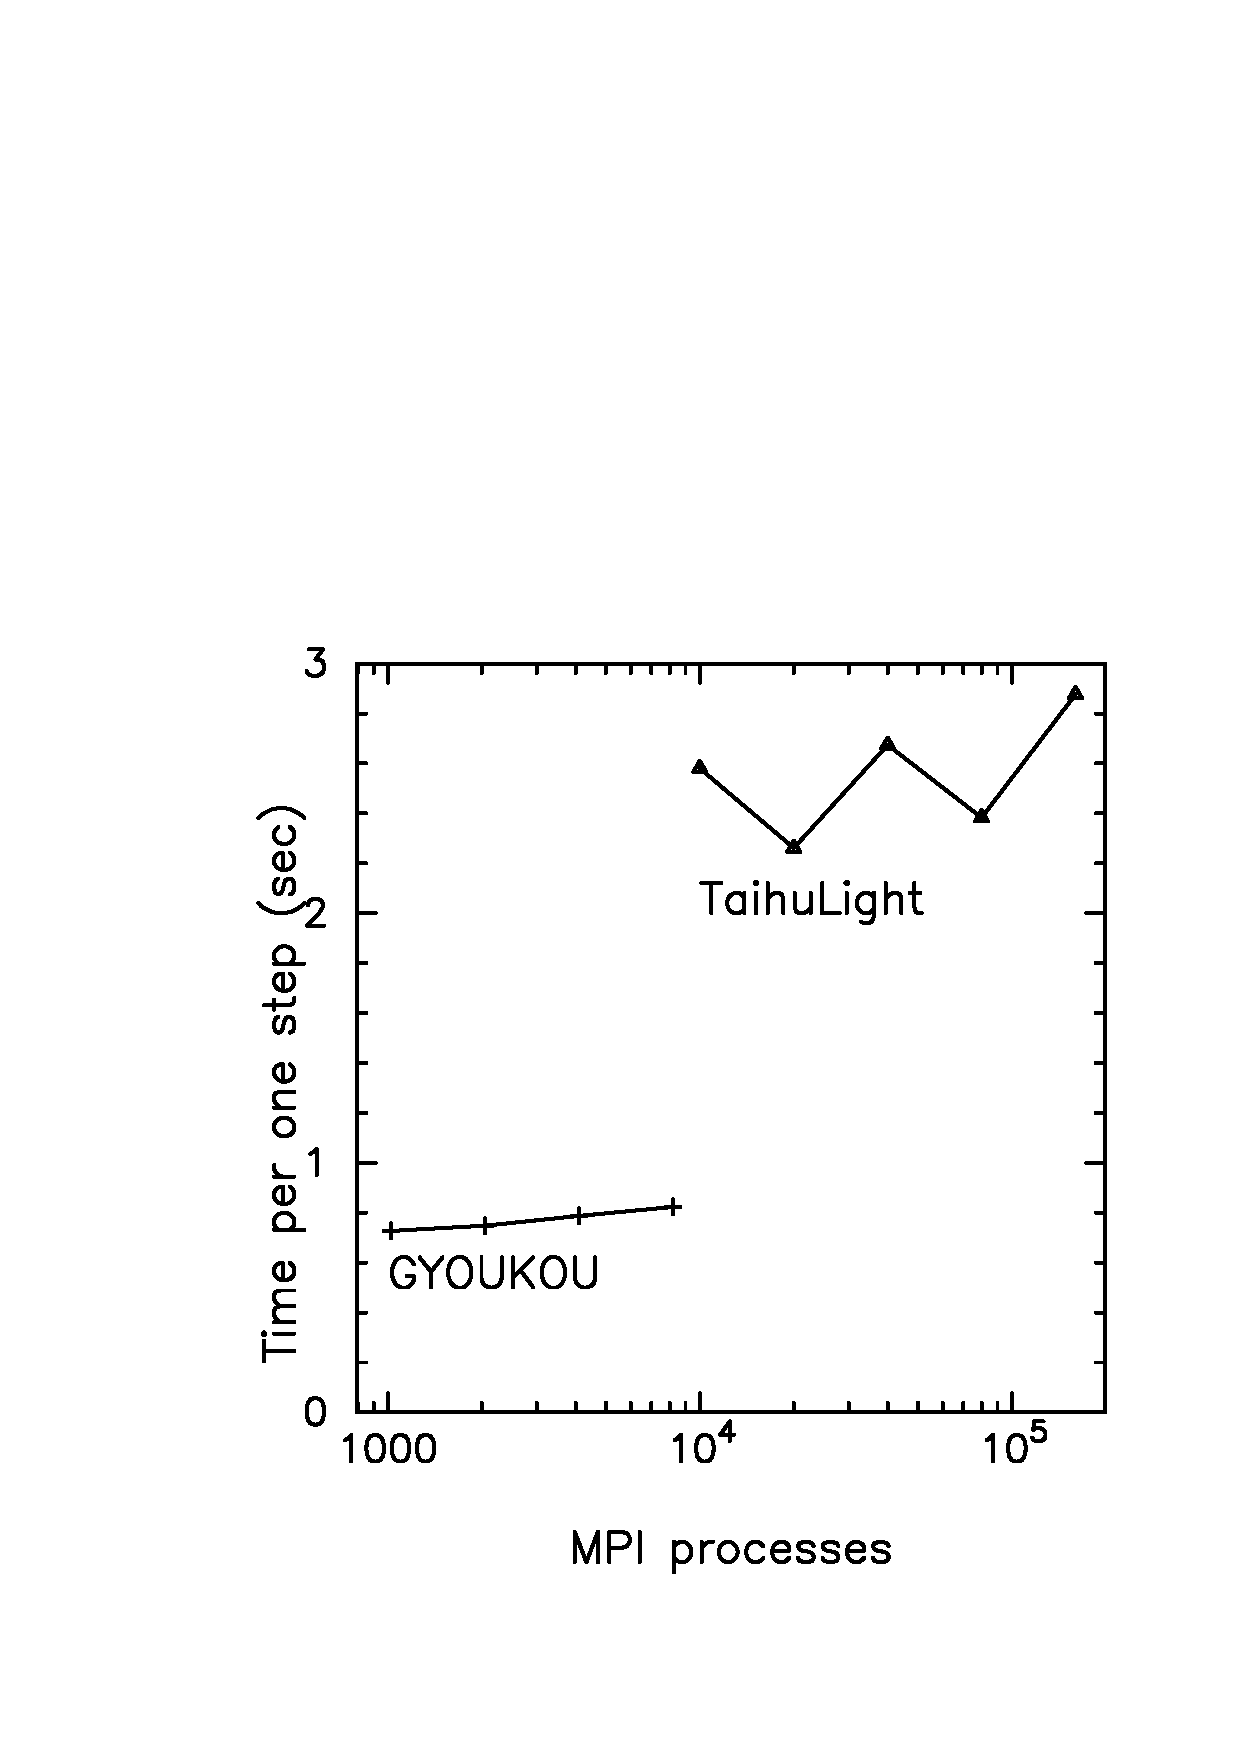
\includegraphics[width=3in]{weak_scaling2}
\caption{Time per timestep for weak-scaling test. The number of
  particles per process is 10M. Triangles and crosses  show the
  results on TaihuLight and GYOUKOU, respectively.
}
\label{fig:weak}
\end{figure}

\begin{figure}
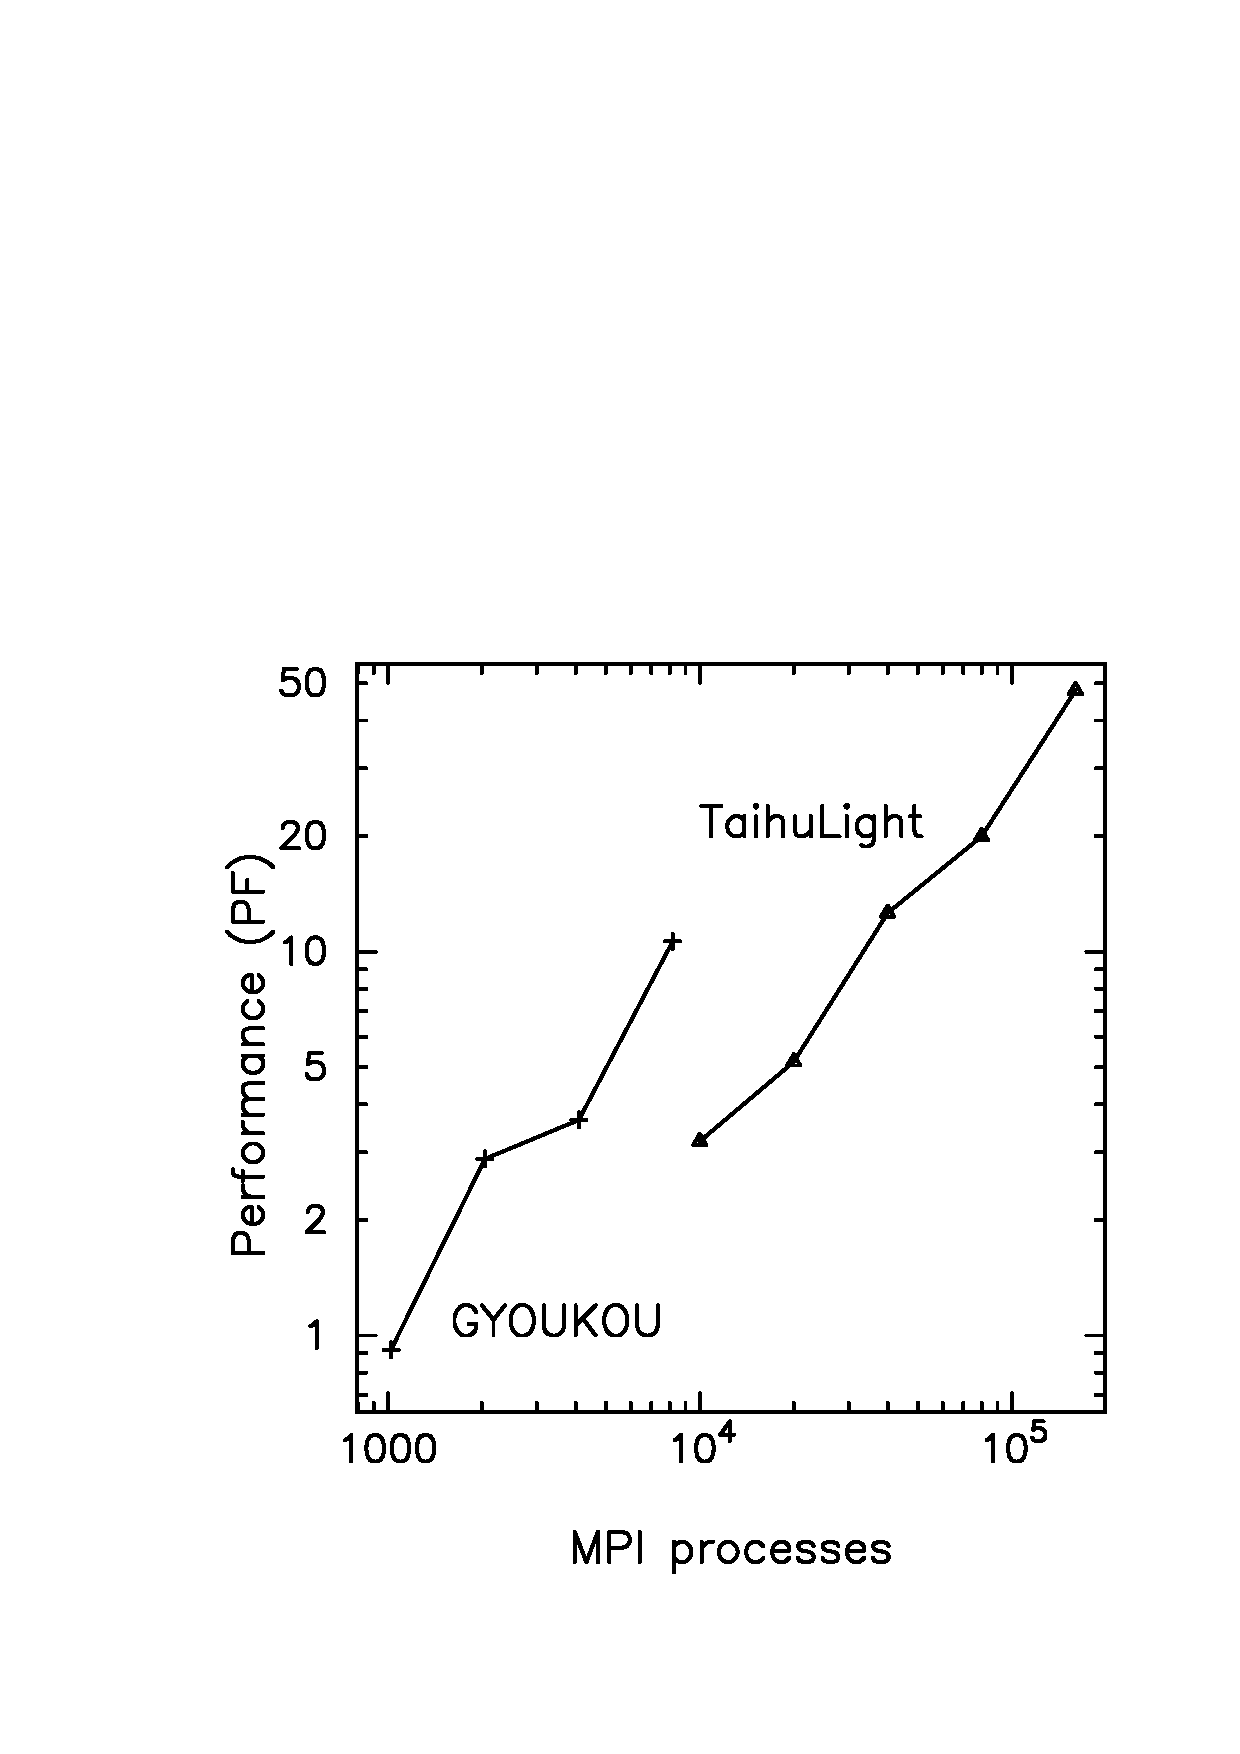
\includegraphics[width=3in]{weak_scaling_speed}
\caption{Performance in petaflops for weak-scaling test.  The number of
  particles per process is 10M. Triangles and crosses  show the
  results on TaihuLight and GYOUKOU, respectively.}
\label{fig:weakpf}
\end{figure}

\begin{figure}
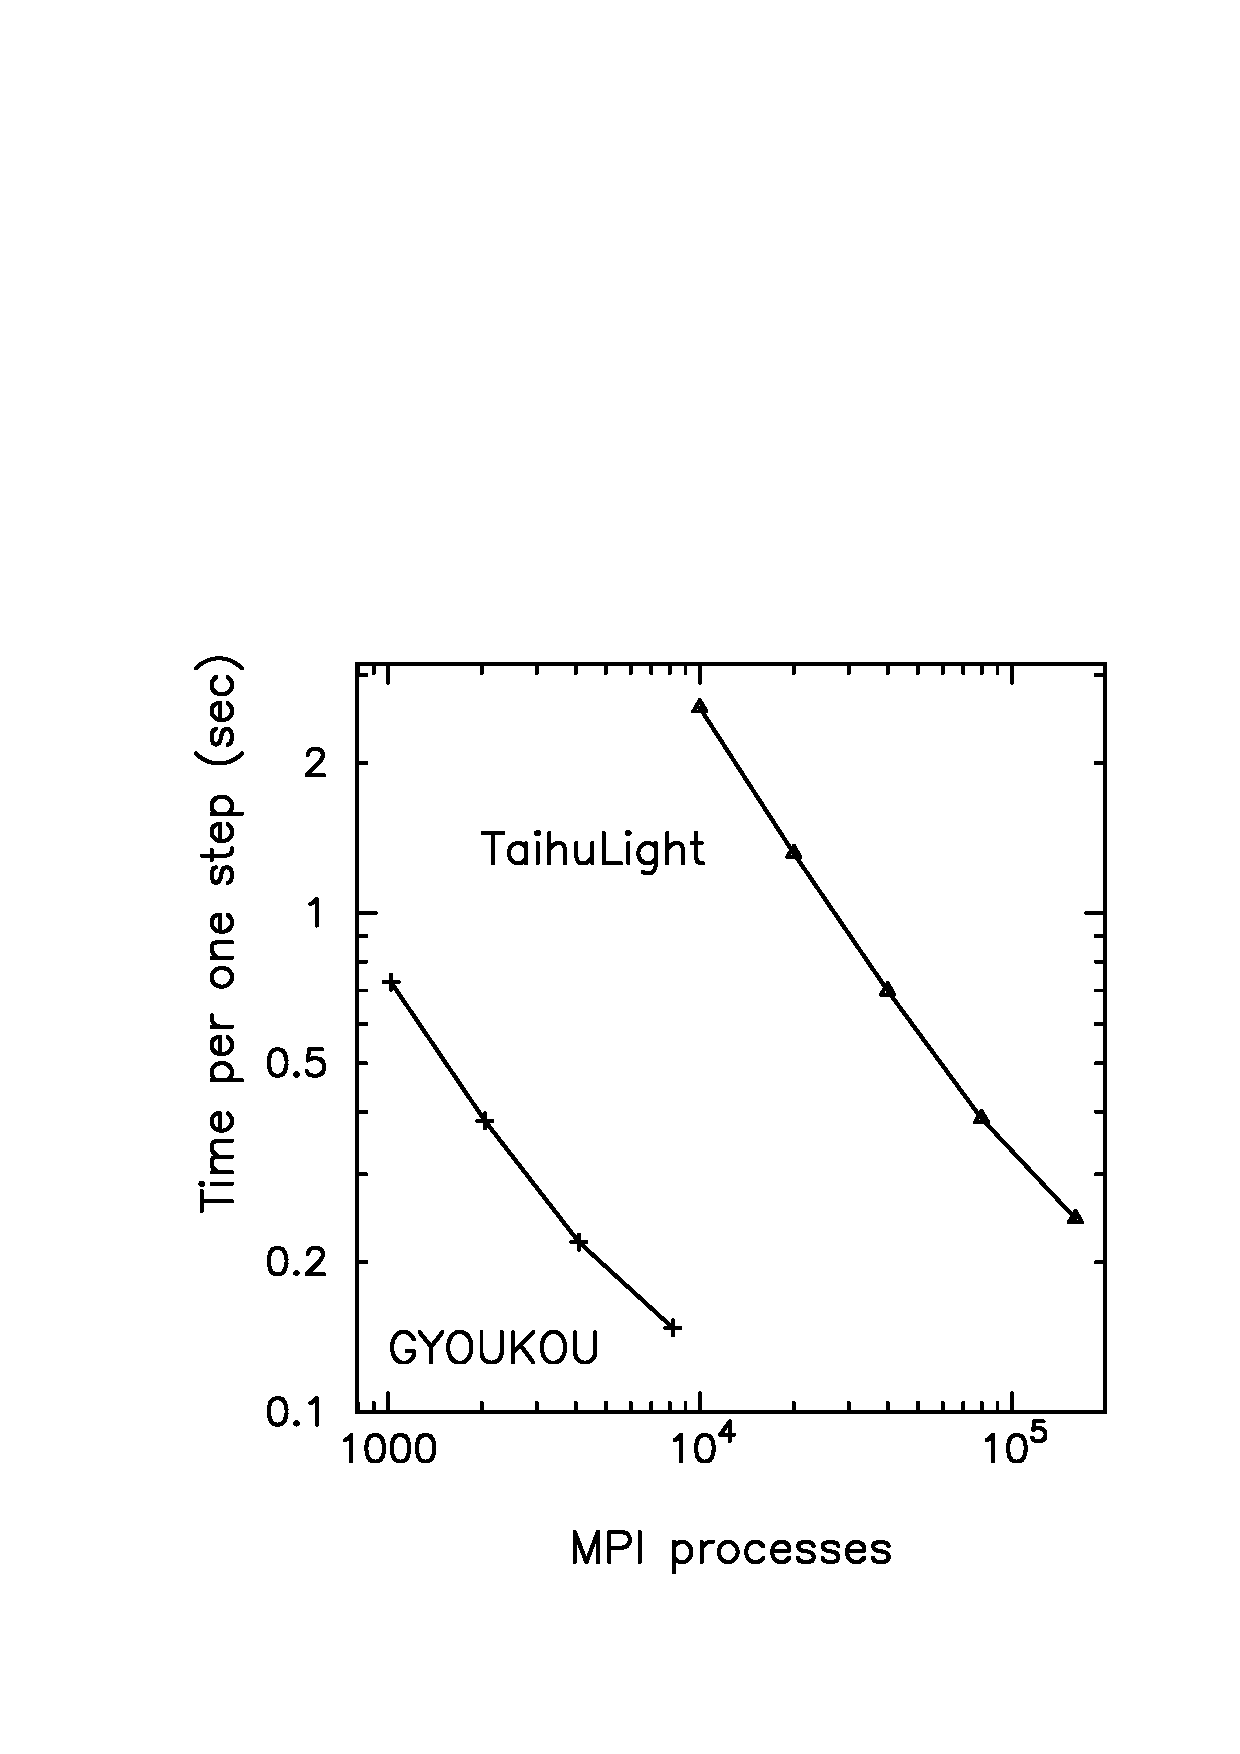
\includegraphics[width=3in]{strong_scaling}
%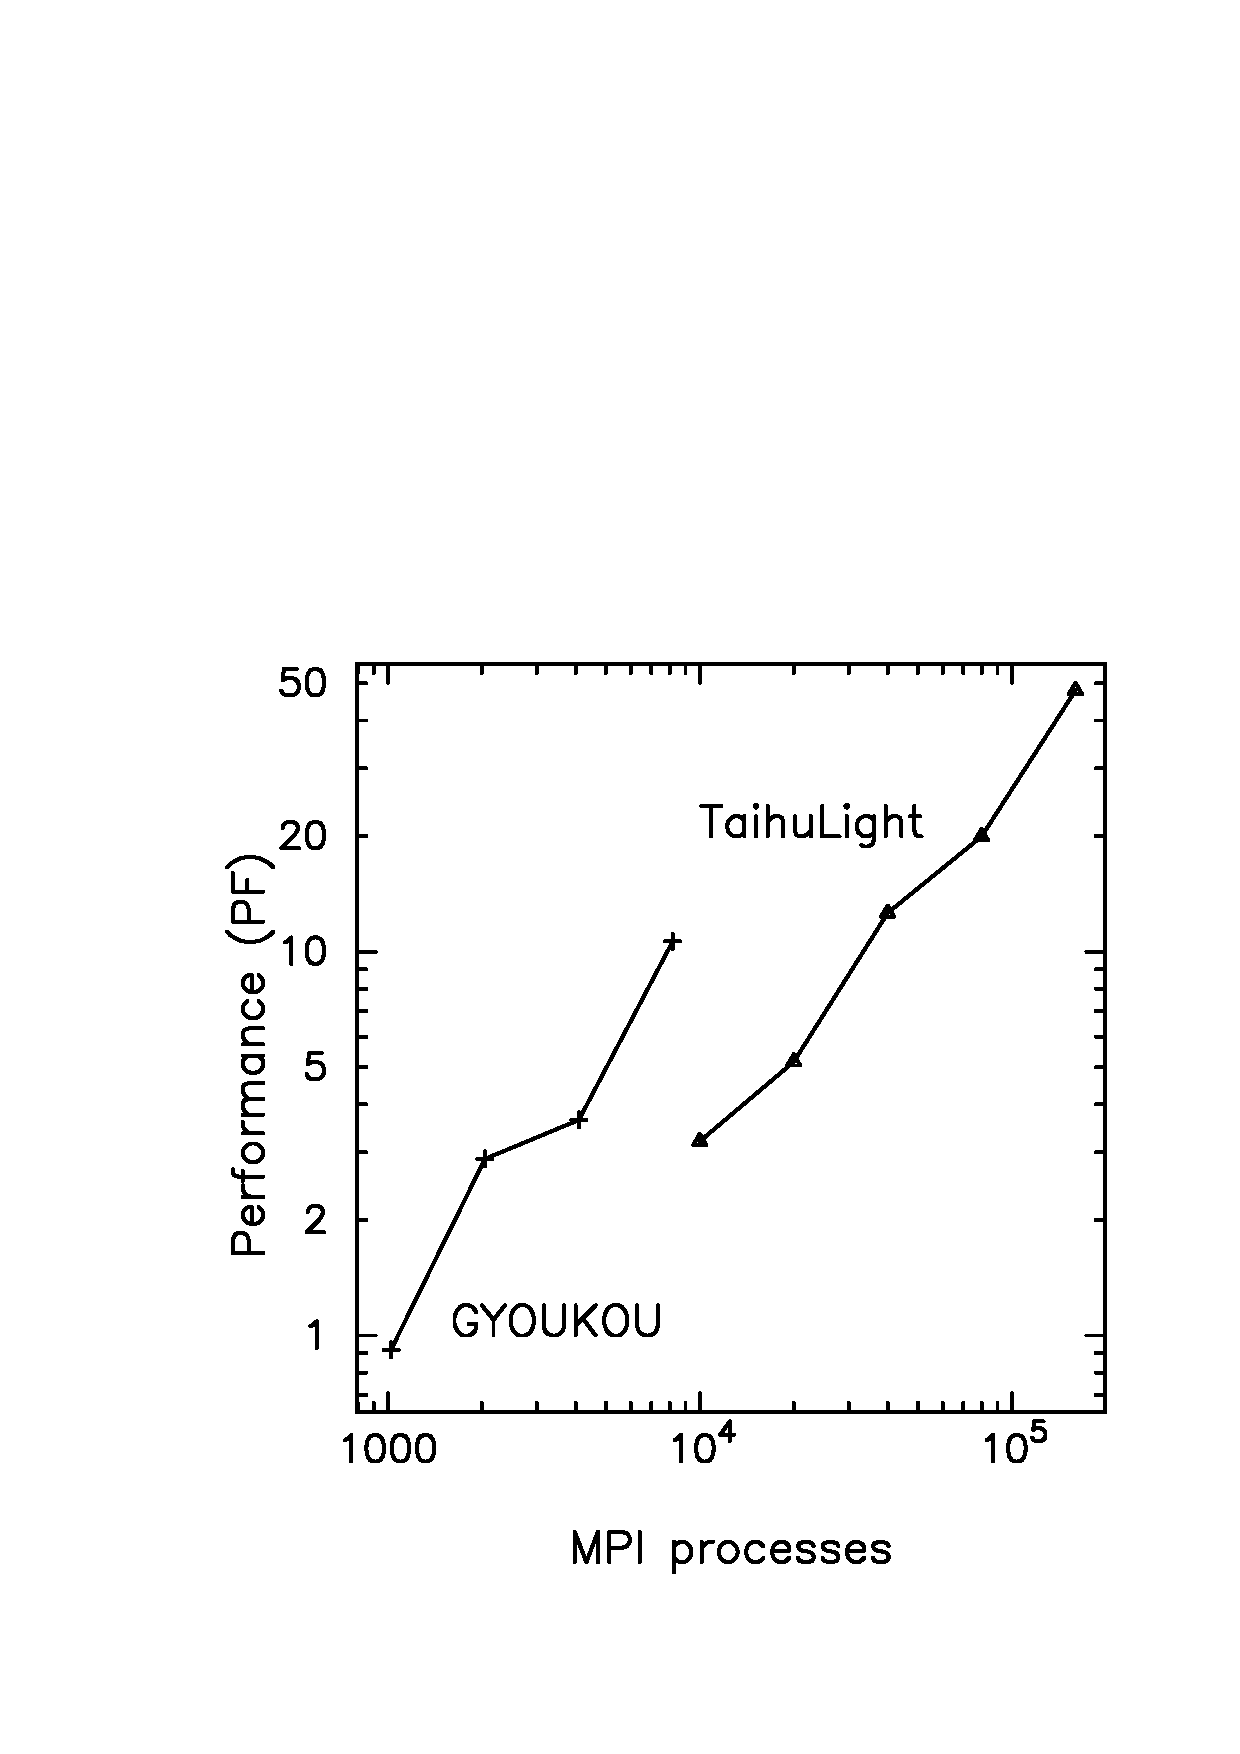
\includegraphics[width=3in]{weak_scaling_speed}
\caption{Time per timestep for strong-scaling test.  Triangles and crosses  show the
  results on TaihuLight and GYOUKOU, respectively. The total number of
  particles is $10^{11}$ on TaihuLight and $10^{10}$ on GYOUKOU.}
\label{fig:strong}
\end{figure}


Figures \ref{fig:weak} and \ref{fig:weakpf}  shows the time per one
timestep and the performance, for the
weak scaling measurements. We can see that the weak scaling
performance is quite good on both of TaihuLight and GYOUKOU. The peak
performance of single MPI process is roughly four times faster for
GYOUKOU, and that's the reason why it is around three times faster in
this weak-scaling measurement. 
Figures \ref{fig:strong} shows the strong scaling result. The total
number of particles is $10^{11}$ and  $10^{10}$, for TaihuLight and
GYOUKOU. We can see that speedup is almost linear.


\begin{table}
\centering
  \caption{Breakdown of calculation time for weak-scaling runs}
  \label{tab:timeweak}
  \begin{tabular}{ccccc}
    \hline
 System  & \# processes & interaction & comm. & others\\
    \hline  
&10000 &   2.07& 0.041 & 0.466\\
&20000 &  1.63& 0.040  & 0.590 \\
TaihuLight &40000  &  2.13 & 0.064 & 0.478 \\
&80000 &   1.71 & 0.053 & 0.630\\
&160000 &  2.31& 0.090& 0.476\\
\hline
&1024&  0.332 &  0.114 & 0.281\\
GYOUKOU &2048&   0.392 & 0.121 & 0.235\\
&4096&  0.355 & 0.143& 0.289\\
&8192   & 0.453& 0.147&     0.222\\
\hline
\end{tabular}
\end{table}

\begin{table}
\centering
  \caption{Breakdown of calculation time for strong-scaling runs}
  \label{tab:timestrong}
  \begin{tabular}{ccccc}
    \hline
 System  & \# processes & interaction & comm. & others\\
    \hline  
& 10000& 2.0738 & 0.0410 & 0.4658 \\
& 20000& 1.0499 & 0.0253 & 0.2426 \\
TaihuLight & 40000& 0.5565 & 0.0298 & 0.1125 \\
& 80000& 0.2991 & 0.0233 & 0.0652 \\
& 160000& 0.1765 & 0.0322 & 0.0356 \\
\hline
& 1024& 0.3323 & 0.1140 & 0.2808 \\
GYOUKOU & 2048& 0.1512 & 0.0668 & 0.1658 \\
& 4096& 0.0854 & 0.0417 & 0.0923 \\
& 8192& 0.0538 & 0.0357 & 0.0582 \\
    \hline  
\end{tabular}
\end{table}
 
Tables\ref{tab:timeweak} and \ref{tab:timestrong} show the breakdown
of the calculation time per one timestep, again for both the weak and
strong scaling runs. As expected, in the case of strong-scaling runs,
the calculation time for communication does not decrease
significantly, and eventually limits the performance.  As already
stated, our main interest is to use very large number of
particles. Therefore, for actual scientific runs, the communication
time would not become the limiting factor.

The performance of run for $1.6\times 10^{12}$ particles on 160k
processes (40000 nodes) of TaihuLight is 47.9 Pflops, or 39.7\% of the
theoretical peak performance of the Sunway TaihuLight system.  On
GYOUKOU, we achieved 10.6 Pflops for $8\times 10^{9}$ particles on 8k SC2
chips, or efficiency of 23.3\% of the theoretical peak performance.

The overall efficiency we achieved on GYOUKOU is a bit lower compared
to that on TaihuLight. This difference is not due to any fundamental
difference in the architecture but purely due to the limitation on the
available time for program development and performance measurement. As
we stated, the calculation in the list-construction step, such as
the constructions of the tree and the interaction lists are currently
done on Xeon~D, and around 40\% of the total time is consumed in this
step. We plan to improve the performance of GYOUKOU soon.

 In terms of the number of
particles integrated per second, we have achieved $5.5\times
10^{11}$ particles per second, which is more than 10 times faster than
the results of previous works on
K computer\cite{Ishiyamaetal2012} or ORNL Titan
\cite{Bedorfetal2014}.

% Bedorfetal 5.5 sec for 242B particles = 
% Ishiyama 2.5e-11 sec/aprticle

\section{Implications}

%  implications for future systems and applications (1 p max)

In this paper, we described the implementation and performance of
a highly efficient simulation code for self-gravitating planetary
rings on  Sunway TaihuLight and GYOUKOU.

The measured performance is 47.9 Pflops, or 39.7\% of the theoretical
peak, for simulation of $1.6\times 10^{12}$ particles on 40,000 nodes
of TaihuLight, and 10.6PF, or 23.3\% of the theoretical peak, for
simulation of $8\times 10^{10}$ particles on 8192 nodes of GYOUKOU.

Compared to previous achievements on K computer or ORNL Titan, the
achieved efficiency is similar or higher, and the speed in terms of
the number of particles integrated per second is higher, for both
TaihuLight and GYOUKOU. As we stated earlier, this level of
performance would not be achieved without the new algorithms described in
this paper. 

Compared to other multi-core processors for modern  HPC systems such
as Fujitsu SPARC64 VIIIfx and IXfx or Intel Xeon Phi processors,
both SW26010 processor  of TaihuLight and PEZY-SC2 processor of
GYOUKOU have several unique features which allow very high peak
performance but at the same time make it much harder to achieve high
efficiency on real applications. These are:
\begin{itemize}

  \item Heterogeneous architecture with rather extreme performance
    ratio of 1:64 in the case of SW26010 and even larger in the case
    of SC2.
  \item The lack of cache hierarchy (SW26060) or cache coherency (SC2).
  \item Very limited main memory bandwidth, with B/F values around
    0.02--0.04.  This is about 1/10 of the numbers of Fujitsu or Intel HPC processors.
    
\end{itemize}  

On the other hand, SW26010 comes with very well-thought features which
allows the programmers to optimize the performance of code on
CPE. These features include:
\begin{itemize}

\item Low-latency DMA controller which can be initiated by any CPE.
\item Low-latency, high-bandwidth communication between CPEs.
  
\end{itemize}  

These two features allow very efficient use of the main memory
bandwidth. The two-dimensional structure of the network within CG seem
to be optimized for highly efficient implementation of matrix-matrix
multiplications, but it is actually quite useful for other real
applications, whenever fast inter-core communication is necessary.

It is certainly true that the need to use DMAs for data transfer
between CPE and main memory complicates the use of CPE. However, it is
also true that it makes quite optimized access to main memory
possible, since the application programmer can (or have to) control
all main memory accesses. In the case of our code, in several places
we have ``vectorizable'' loops, which perform the same operation on all
particles in the system. The number of operations per particle is
relatively small, of the order of ten, and the data size of one
particle is 32 bytes. In the case of manycore architecture with
hierarchical cache memory, to achieve high efficiency on simple vector
operations like 
\\
{\tt \hspace*{1em} a[i] =   b[i]+c[i]}
\\
is actually quite complicated. In modern processors, load address
would be predicted and hardware prefetch is generated. The hardware
prefetch would probably work for a very simple loop like the above
example, but would fail if many vectors are loaded. Then the
programmer need to experiment with software prefetch, to find the way
to get  the best performance. 

In the case of SW26010, currently it is rather tedious and error-prone
to write the equivalent operation using the combination of {\tt Athread}  and
DMA, and sometimes inner kernel in assembly language, but once we do
so, we can get a performance close to the theoretical limit
relatively easily.

The existence of low-latency (less than 10 clock cycles) communication
path between CPEs is quite important for using CPEs for fine-grain
parallelism such as loop-level parallelization. Such low-latency
communication is difficult to implement on shared memory processors
with hierarchical cache.

The SC2 processor supports the cache flash and
synchronization at each level of the cache hierarchy, making the
relatively low-latency communications between processors possible.
However, it is clearly desirable to have  more direct control of
interprocessor communication.

One  problem with the current software/hardware system is that writing
high-performance kernel for SW26010 or SC2  currently means writing the inner
kernel in the assembly language. This is purely the software limitation,
and probably not so difficult to fix. In this aspect, SC2 is somewhat
easier to deal with, since it supports 8-way multithreaded execution,
which effectively hides the latencies of L1 cache and arithmetic unit
from compiler. 



In conclusion, we have implemented parallel particle simulation code
on Sunway SW26010 and PEZY-SC2 processors, and found that it is not
impossible to achieve high performance on their rather extreme
architectures with carefully designed algorithms. Even though the B/F
number are less than 0.1  and the network bandwidth is similarly low, the efficiency we
have achieved is comparable to that on K computer, with 15
times more memory and network bandwidth. We feel that architecture
evolution in this direction will help the HPC community to continue
improving the performance.





% conference papers do not normally have an appendix


% use section* for acknowledgment
\section*{Acknowledgment}


This work was supported in part by The Large Scale Computational
Sciences with Heterogeneous Many-Core Computers in grant-in-aid for High
Performance Computing with General Purpose Computers in MEXT (Ministry
of Education, Culture, Sports, Science and Technology-Japan) and  also
in part by  JAMSTEC, RIKEN, and PEZY Computing,
K.K./ExaScaler Inc.
In this research computational resources of the GYOUKOU supercomputer,
developed under the ``Large-scale energy-efficient supercomputer with
inductive coupling DRAM interface'' project of NexTEP program of Japan
Science and Technology Agency, has been used.







% trigger a \newpage just before the given reference
% number - used to balance the columns on the last page
% adjust value as needed - may need to be readjusted if
% the document is modified later
%\IEEEtriggeratref{8}
% The "triggered" command can be changed if desired:
%\IEEEtriggercmd{\enlargethispage{-5in}}

% references section

% can use a bibliography generated by BibTeX as a .bbl file
% BibTeX documentation can be easily obtained at:
% http://mirror.ctan.org/biblio/bibtex/contrib/doc/
% The IEEEtran BibTeX style support page is at:
% http://www.michaelshell.org/tex/ieeetran/bibtex/
%\bibliographystyle{IEEEtran}
% argument is your BibTeX string definitions and bibliography database(s)
%\bibliography{IEEEabrv,../bib/paper}
%
% <OR> manually copy in the resultant .bbl file
% set second argument of \begin to the number of references
% (used to reserve space for the reference number labels box)
%% \begin{thebibliography}{1}

%% \bibitem{IEEEhowto:kopka}
%% H.~Kopka and P.~W. Daly, \emph{A Guide to \LaTeX}, 3rd~ed.\hskip 1em plus
%%   0.5em minus 0.4em\relax Harlow, England: Addison-Wesley, 1999.

%% \end{thebibliography}

\bibliographystyle{IEEEtran}


\bibliography{allrefs}




% that's all folks
\end{document}


